\chapter{Implementace}
\label{chap:implementation}
Celý systém pro správu kampaní je rozdělen do několika celků. Základem je webový server, postavený na frameworku Next.js, který zprostředkovává komunikaci mezi dalšími častmi.
Pracovní postup se systémem je následnový:
\begin{enumerate}
    \item import dat,
    \item úprava ve webovém rozhraní,
    \item exportování dat a použití v reklamním systému.
\end{enumerate}
Data jsou perzistována v relační databázi PostgreSQL pomocí ORM systému Prisma.
Paměťové úložiště v databázi Redis slouží jako zprostředkoval pro frontu úloh (Celery), cacheování požadavků na API třetích stran a dočasné úložiště importovaných dat.

\begin{figure}[h]
    \centering
    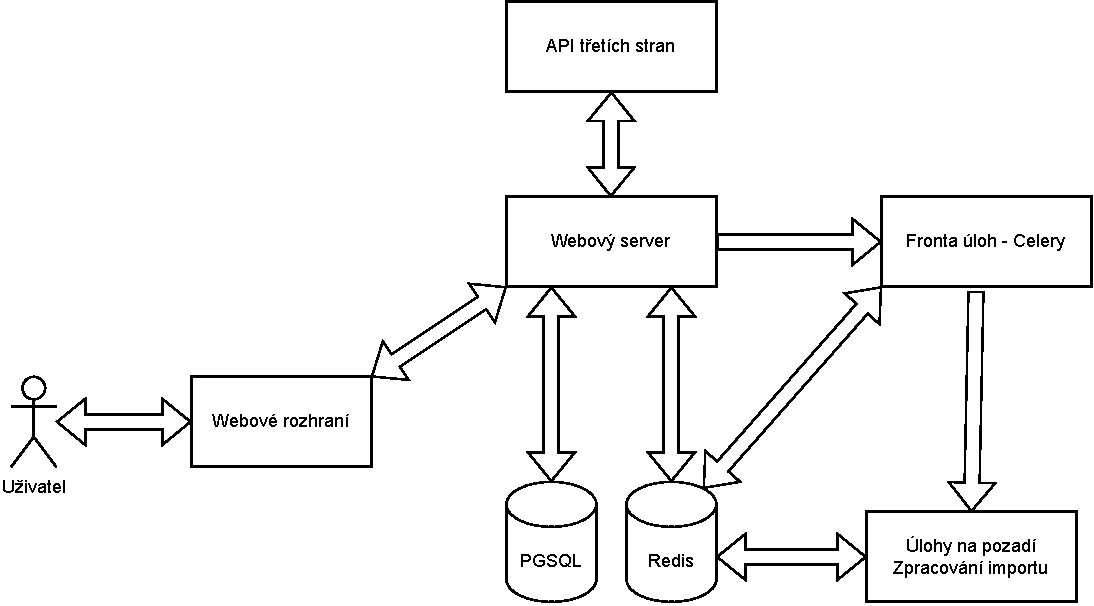
\includegraphics[width=1\textwidth]{Figures/system-overview.pdf}
    \caption{Náhled systému}
    \label{fig:system-overview}
\end{figure}

\section{Importování souborů}
Ve webovém rozhraní, které slouží jako hlavní způsob interakce systému s uživatelem, je umožněno vybírání souboru ke zpracování.
Jakmile je tento soubor nahrán na server, vytvoří se nový úkol do fronty úloh. Na pozadí je automaticky spuštěň nový proces, který
zpracovává nahraný soubor. Uživatele v tento moment nic neblokuje a nebrání s další interakcí se systémem.

CSV soubory využívané pro export/import kampaní se řídí pravidlem každé položky na samostatném řádku. \cite{sklik:csv} Nejjednodušší představa, o tomto pravidle je takové, že
každá položka ma svůj klíčový sloupec, pomocí kterého lze rozeznat rozeznat typ položky. Jesliže tedy v CSV souboru existuje sloupec \enquote{Keyword} a v tomto sloupci je
na nějakém řádku hodnota, bude celý tento řádek popisovat klíčové slovo. Podobně, pokud například existuje sloupec \enquote{Headline 1} a v na nějakém řádku 
je v tomto sloupci hodnota, bude celý řádek popisovat textovou reklamu. Pár výbraných klíčových sloupců a co popisují lze vidět v tabulce \ref{tab:csv-columns}.
Jesliže je na stejném řádku ve více takovýchto sloupců hodnota, je to považováno za chybu a nelze takovýto řádek importovat. Jedinou výjimkou jsou sloupce
\enquote{Campaign} a \enquote{Ad Group}, které v dané situaci nabývají významu, ke které kampani a sestavě daná reklama či klíčové slovo patří.

\begin{table}[h]
    \centering
    \begin{tabular}{ |l|l| }
        \hline
        Označení sloupce & Typ položky \\
        \hline
        Campaign & Kampaň \\
        Ad Group & Sestava \\
        Keyword & Klíčové slovo \\
        Age & Cílení - věk \\
        Gender & Cílení - pohlaví \\
        Topic & Cílení - Téma \\
        Image & Banner \\
        Headline 1 & Textová reklama \\
        \hline
    \end{tabular}
    \caption{Tabulka klíčových sloupců a označení typů položky CSV souboru reklamních kampaní}
    \label{tab:csv-columns}
\end{table}

Záhlaví sloupců je vyžadováno, jinak nelze poznat, co bude který řádek popisovat.

Importovaný soubor nemusí být jen jednotlivý CSV soubor, ale taktéž ZIP archiv, který tento CSV soubor obsahuje.
Výhoda archivního souboru spočívá v možnosti nahrát si do systému i své bannery. K tomu je nutné, aby
v archivu existovala složka s název \enquote{banners}, ve které budou obrázkové soubory. Tyto bannery se uloží na serveru a zároveň
je k nim vytvořen záznam do databáze. Bannery se mohou nahrát do systému i samostatně, bez nutnosti využití importovacího rozhraní.


Jakmile jsou data ze souboru získána, jsou dočasně uloženy do paměťové databáze Redis a uživateli je zobrazeno upozornění.
Po rozkliknutí je přesměrován na stránku \ref{fig:import-sar}, kde si může vybrat, které části si přeje importovat a které ne.

\begin{figure}[h]
    \centering
    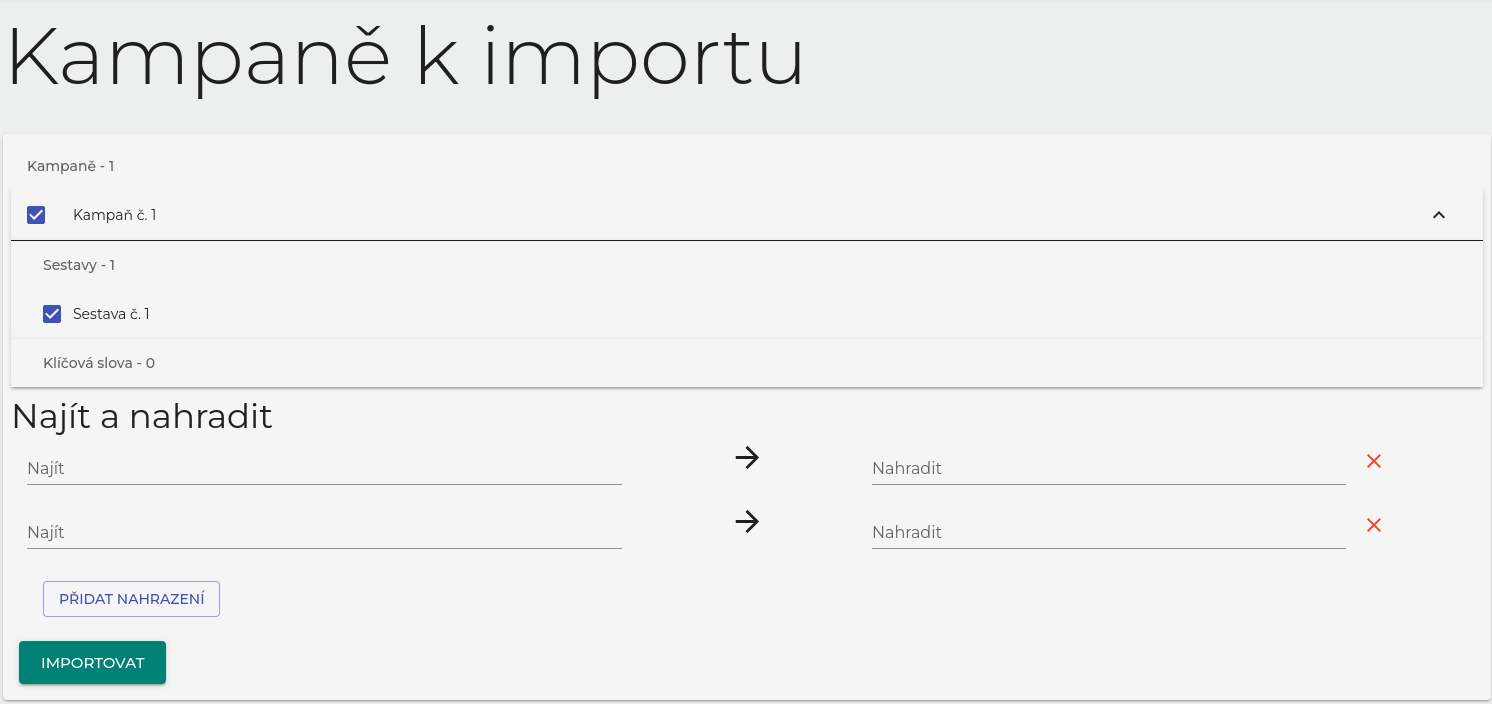
\includegraphics[width=1\textwidth]{Figures/ui/import-sar.png}
    \caption{Rozhraní pro importování kampaní a metadat}
    \label{fig:import-sar}
\end{figure}

Další možností, kterou lze v tomto mezikroku využít je funkce najít a nahradit. Uživatel si může přidat libovolné množství
slov, která chce najít a nahradit. V případě využití této funkce se spustí další úloha na pozadí, která tento požadavek splní.
Následně jsou data zapsaná do relační databáze. Pokud se při zapisování reklamních dat objeví hodnota ve atributu \enquote{Image},
je daný záznam propojen se záznamem o nahraném banneru.

Na třídním diagramu \ref{fig:campaigns-class-diagram} je vidět struktura kampaní, do které jsou data z CSV souboru transformována. Třída \emph{Targeting} reprezentuje všechny
možné typy cílení, které se mohou v CSV vyskytovat (věk, pohlaví, \ldots). 

\begin{figure}[h]
    \centering
    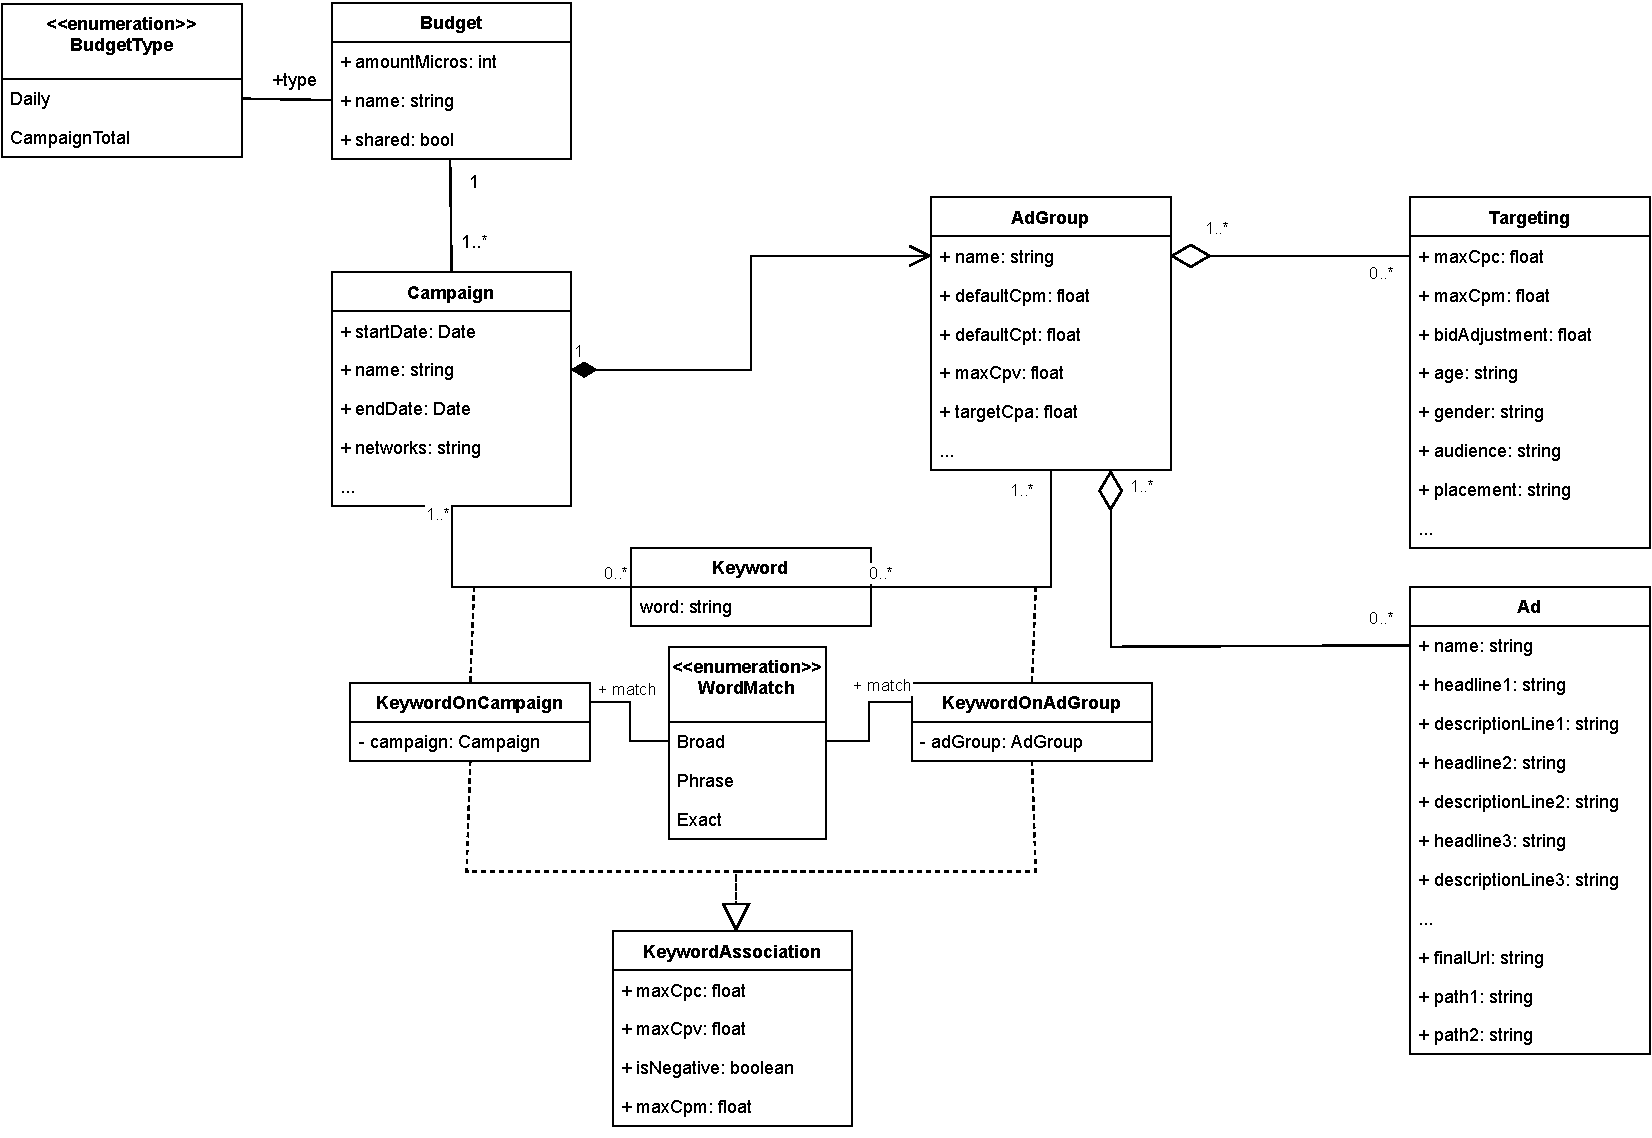
\includegraphics[width=1\textwidth]{Figures/campaigns-class-diagram.pdf}
    \caption{Třídní diagram sturktury kampaní}
    \label{fig:campaigns-class-diagram}
\end{figure}


\section{Tabulková správa kampaní}
Jak již bylo zminěno v části \ref{subsec:edit-campaigns}, jedním z nejrychlejších způsobu editace kampaní je tabulkovým procesorem.
Proto bylo ve webovém rozhraní vytvořena možnost pracovat podobným způsobem. Obrázek \ref{fig:datagrid-window} ukazuje celkový pohled na rozhraní, ve kterém uživatel
může provádět úpravy a správu svých kampaní a metadat.

\begin{figure}[h]
    \centering
    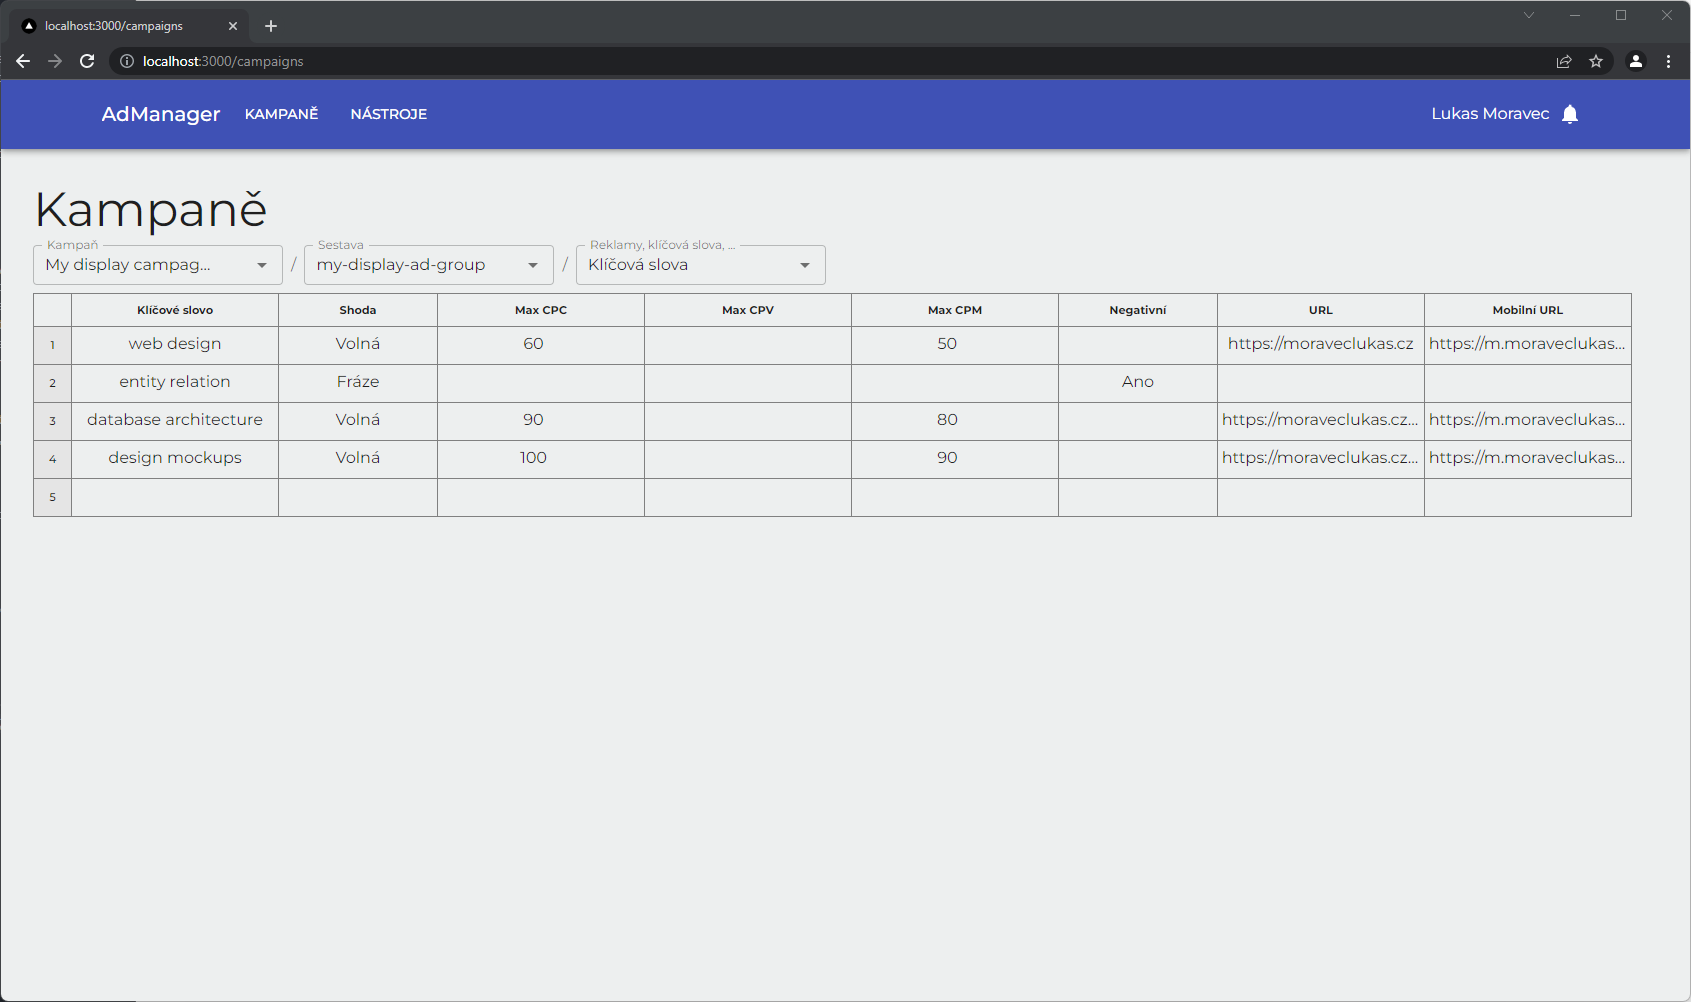
\includegraphics[width=1\textwidth]{Figures/ui/whole-window.png}
    \caption{Pohled na webové rozhraní umožňující správu kampaní}
    \label{fig:datagrid-window}
\end{figure}
Hlavní částí je komponenta \emph{DataGrid} (\ref{fig:datagrid}).
\begin{figure}[h]
    \centering
    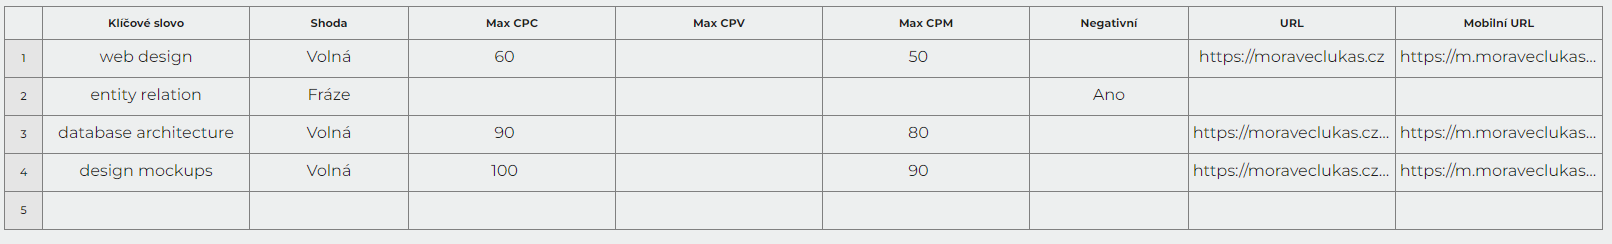
\includegraphics[width=1\textwidth]{Figures/ui/datagrid.png}
    \caption{Komponenta DataGrid}
    \label{fig:datagrid}
\end{figure}
Ta jako svůj vstup vyžaduje definici jednotlivých sloupců
a pak samotná data. Definice sloupců obsahuje jeho datový typ, případně taky seznam možností, ze kterých si uživatel bude moct vybrat svou požadovanou hodnotu.
Tato funkcionalita je znázorněna na obrázku \ref{fig:cell-choices} a jeji využití spočívá převážně u sloupců, jenž mají jednoznačně definované možné hodnoty. DataGrid
dále poskytuje jednoduché duplikování\footnote{Klávesa ALT a dvojité D} a mazání\footnote{Klávesa ALT a dvojité X} záznamů dalšími klávesovými zkratkami. 

Vykreslování tabulkových dat a tabulek bývá výpočetně drahá operace, obzvláště v knihovně React. Jakákoliv změna stavu dat, tedy jakýkoli uživatelský vstup, by způsoboval
překreslení celé tabulky. Aby se zamezilo nadměrnému vykreslování, existují 2 metody, které lze využít pro zlepšení výkonu. První z nich se nazývá \emph{debouncing}. V podstatě se jedná
o funkci s nastaveným prahem\footnote{Nastavený prah je časová hodnota, nejčastěji udávána v milisekundách. Závisí však na konkrétní implementaci},
která zachytává události (a nepropouští dále) nějakého typu (např. uživatelský vstup). Jestliže v nastavené době \textbf{nenastane událost}, vyšle poslední zachycenou.

Druhá metoda pro optimalizaci vykreslování je memoizace. Při interakci uživatele s DataGridem se vždy mění obsah jedné buňky, respektive 2 buněk při změně zvýrazněné buňky.
React toto neví a překresluje celou tabulku. Naštěstí můžeme buňky memoizovat, díky čemu překreslení nastane překreslení jen a pouze té buňky, která to doopravdy potřebuje.


\begin{figure}
    \begin{minipage}{.5\textwidth}
        \centering
        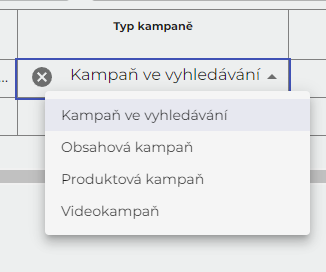
\includegraphics[width=.7\textwidth]{Figures/ui/cell-choices.png}
        \caption{Výběr možností}        
        \label{fig:cell-choices}
    \end{minipage}
    \begin{minipage}{.5\textwidth}
        \centering
        
\includegraphics[width=1\textwidth]{Figures/ui/datagrid-controls.png}
        \caption{Navigační prvky DataGridu}        
        \label{fig:datagrid-controls}
    \end{minipage}
\end{figure}

Pro jednoduchou a hlavně rychlou orientaci mezi kampaněmi, sestavamy, klíčovými slovy a reklamami slouží trojice Select boxů (obrázek \ref{fig:datagrid-controls}) s automatickým filtrováním.
Každý Select má svou klávesovou zkratku, skrze kterou se dá s daným vstupem ihned interagovat. 



\subsection{Automatické ukládání změn}
Všechny provedené změny se automaticky ukládají pomocí technologie \emph{Websockets}. Ta zprostředkovává plně duplexní komunikační kanál mezi serverem a prohlížečem uživatele.
Websocket na serverové straně také umožňuje vzniklé události přeposílat všem připojeným klientům metodou broadcast. Tato spojení lze rozlišit podle přihlášeného uživatele nebo jakýchkoli jiných
kritérií. Díky onomu přeposílání událostí je možné, aby na správně kampaní pracovalo více uživatelů najednou a v reálném čase viděli všechny prováděné změny.

\begin{figure}[h]
    \centering
    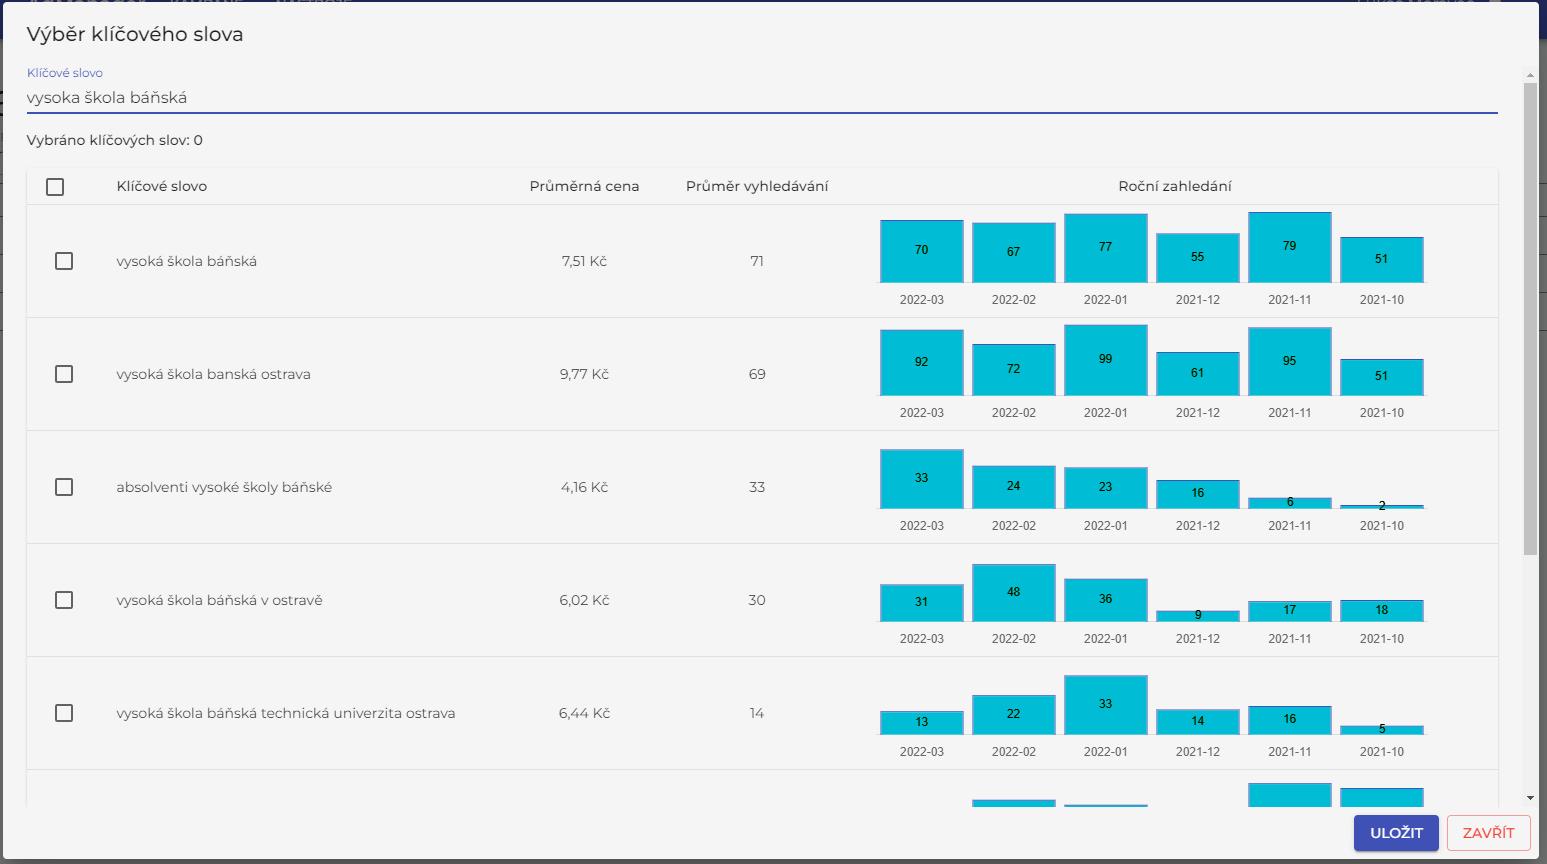
\includegraphics[width=1\textwidth]{Figures/ui/keyword-dialog.png}
    \caption{Dialogové okno pro výběr klíčových slov}
    \label{fig:keyword-dialog}
\end{figure}

\subsection{Výběr klíčových slov}
Pokud si uživatel ke svému účtu uloží API klíč k platformě Sklik, může využívat doporučování klíčových slov. Stisknutím kláves CTRL a šipky nahoru se otevře dialogové okno,
znázorněné na obrázku \ref{fig:keyword-dialog}. Zobrazí různé návrhy klíčových slov, včetně průměrné ceny za proklik při reakci na klíčové slovo a také počet zahledání, až půl roku zpětně.
Lze vybrat více klíčových slov najednou. Pokud se tak stane, vytvoří se nové záznamy klíčových slov s totožnými parametry, které měl aktuálně nastaven upravovaný záznam.  


\subsection{Validace dat}
Aby byl uživatel upozorněn na to, kdy zádává nevhodnou kombinaci hodnot, byly vytvořeny validátory, znázorněné na třídním diagramu \ref{fig:validators}. Každý konkrétní validátor
očekává, že k validaci dostane instanci svého typu. Některé objekty potřebují ke správné validaci vědět, zda jsou součástí kampaně nebo sestavy správného typu.
Jakmile nastane nějaká změna, je celý záznam vždy znovu validován a chyby jsou uživateli zobrazeny tak, aby si je mohl opravit.

\begin{figure}[h]
    \centering
    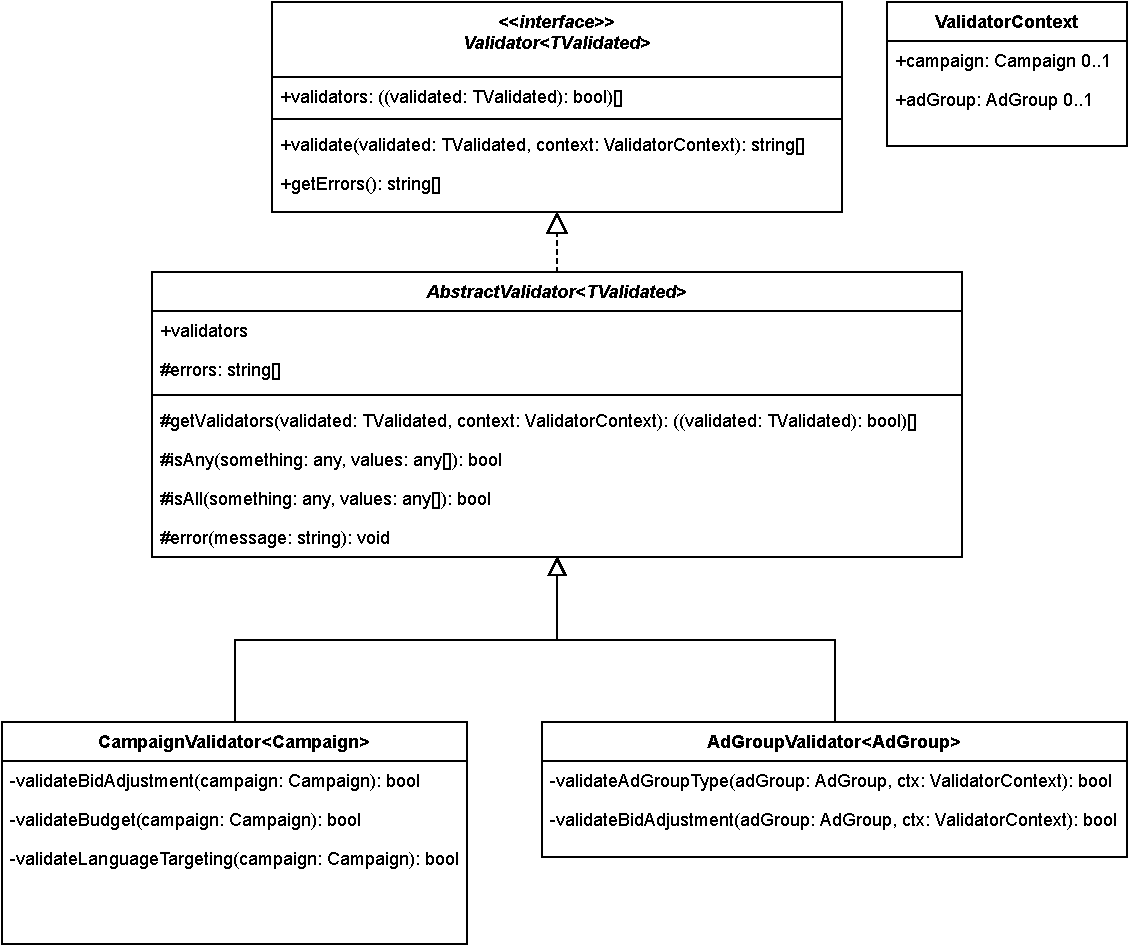
\includegraphics[width=.8\textwidth]{Figures/Validators.pdf}
    \caption{Třídní diagram validátorů}
    \label{fig:validators}
\end{figure}

\section{Transformace XML feedů}
Pro produktové kampaně využívající XML feed je možné využít transformací XML feedů. Transformace jsou podmíněne, tzn. uživatel si vybere podmínku a akci, která se má
vykonat, jesliže je podmínka splněna. Ku příkladu, pokud pole popisující poček kusů na skladu obsahuje nulu, tak je položka z feedu odstraněna. Transformací feedů
se docílí tak, že uživatel zadá adresu svého neupraveného feedu. Systém si tento feed může pravidělně stahovat a provádět na něm transformace. Následně je tento upravený
feed vystavený na nové adrese, kterou uživatel zadá do inzerentního systému. K dispozici jsou podmínky:
\begin{itemize}
    \item větší než,
    \item menší než,
    \item rovná se,
    \item obsahuje.
\end{itemize}
Na tyto podmínky navazují akce:
\begin{itemize}
    \item nahradit,
    \item odstranit,
    \item odstranit element,
    \item zvýšit,
    \item snížit.
\end{itemize}
Akce \enquote{odstranit} odstraní položku feedu splňující danou podmínku, zatímco akce \enquote{odstranit element}
odstraní vybraný XML element položky.


\section{Export kampaní}
% Exportování s bannery
Exportování probíhá podobným způsobem jako import. Ve webovém rozhraní si uživatel vybere kampaně k exportování a může znovu využít funkce najít a nahradit.
Následně se spouští proces na pozadí v Celery frontě se všemi potřebnými daty. V onom procesu probíhá transformace strukturovaných dat do
formátu CSV. O tento převod se stará hierarchie tříd (\ref{fig:transformers}), využivající návrhový vzor \emph{template method}.
Abstraktní třída \emph{AbstractTransformer} definuje kostru konverzního algoritmu a každá odvozená podtřída pouze upravuje specifické
kroky. Strukturovaná data reklamní kampaně jsou transformátorům předána jako slovníky s názvem atributu a jeho hodnotou.
Při převádění dat se nejdříve vytvoří pole o takové délce, kolik sloupců se bude muset zapsat do exportovaného CSV souboru. Informace o tom, jaké sloupce
se budou zapisovat a na které pozici v poli se nachází, se udržuje ve třídě \emph{TransformerContext}. O tomto kontextu ví všechny transformátory.
Postupně se prochází všechny atributy slovníku, které se překládají na sloupec CSV souboru a hodnoty se vkládají do pole.
Jesliže se narazí na nový sloupec, je momentální pole rozšířeno a do kontextového slovníku je připsán záznam o názvu sloupce a jeho index. 
Tímto je zajištěno, že se stejný sloupec nebude nacházet v exportovaném CSV vícekrát.


Pokud se při exportování zjistí, že se exportují taktéž bannery, nebude výstupem pouhý CSV soubor, ale ZIP archiv obsahující daný CSV, společně s bannery.
Tento archiv je možné importovat do reklamního systému Sklik.

\begin{figure}[h]
    \centering
    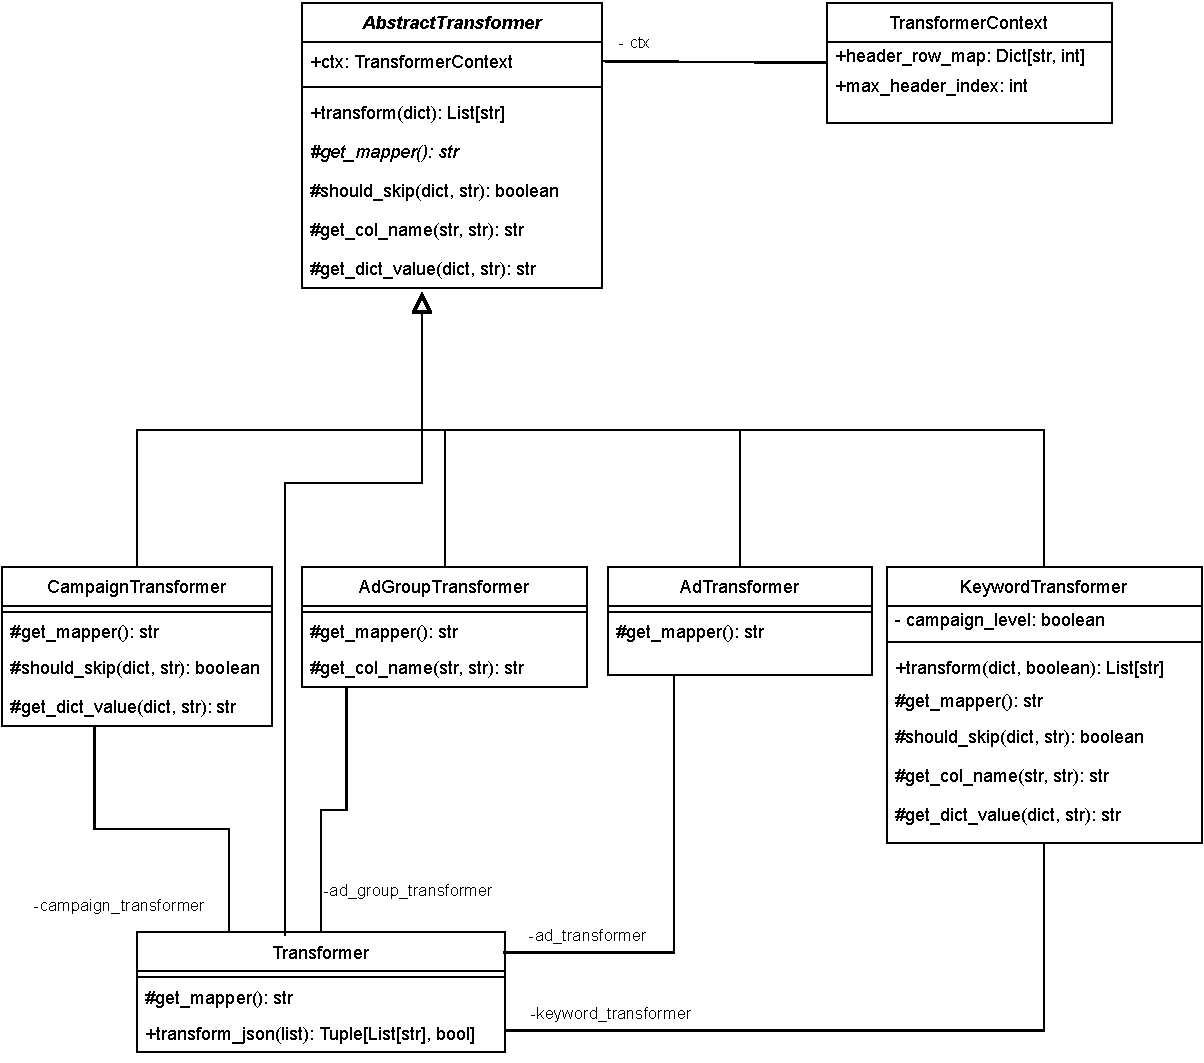
\includegraphics[width=.8\textwidth]{Figures/Transformers.pdf}
    \caption{Třídní diagram transformátorů}
    \label{fig:transformers}
\end{figure}


\endinput